% Example LaTeX file that uses statistics produced by stats.Rnw

\documentclass{article}
%\usepackage{fullpage}
\usepackage{graphicx}
\usepackage{xspace}

\author{Edward J. Schwartz \and Thanassis Avgerinos}
\title{Ed or Thanassis: Which takes longer to type?}

\input{stats}

\begin{document}
\maketitle

In this paper, we analyze which name takes longer to type: Ed or
Thanassis.  We performed \numsamples samples in total to determine
which takes longer.  Our experiments show that Ed takes \edmean
seconds to type on average, compared to Thanassis, which takes
\thanassismean seconds on average.  This can be seen in
Figure~\ref{fig:hist}.

\begin{figure}
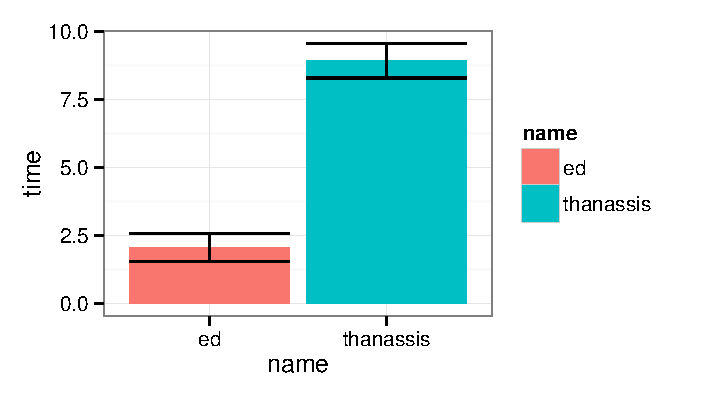
\includegraphics[width=\textwidth]{histsummary.pdf}
\caption{The sample mean time it takes to type Ed and Thanassis in
  \numsamples samples.  Error bars show 95\% confidence interval.}
\label{fig:hist}
\end{figure}

\end{document}

%%% Local Variables: 
%%% mode: latex
%%% TeX-master: t
%%% End: 
